\chapter{应用层}

\noindent\textbf{本章要解决的问题。} 网络应用由运行在端系统上的程序提供。为了让不同主机上的应用交换信息，需要规定应用程序如何寻址彼此、消息按什么格式组织、请求和响应何时发生，并选择能够满足应用需要的传输服务。本章沿课件顺序学习网络应用体系结构、进程通信、DNS、FTP、电子邮件、Web、P2P和Socket API。

\section{网络应用体系结构}
\subsection{客户机/服务器结构}
\textbf{网络应用}是运行在端系统上的程序，例如浏览器、邮件客户端和Web服务器。客户端与服务器是一次应用通信中的两个角色：\textbf{客户机（client）}发起请求并使用服务；\textbf{服务器（server）}等待请求、处理请求并返回结果。它们都是主机上运行的进程，不是专指某种硬件。

在\textbf{客户机/服务器结构（Client--Server，C/S）}中，服务器通常长期在线并有固定、可查找的地址；它可以用多台服务器提供服务和扩展处理能力。客户机间歇性接入网络，地址可能变化，并通过服务器取得服务；典型Web访问中，浏览器向Web服务器发送\textbf{超文本传输协议（HyperText Transfer Protocol，HTTP）}请求，服务器把页面对象作为响应发回。

这种结构容易集中管理，但服务能力受到服务器计算能力和网络带宽限制；服务器故障也可能使许多客户无法使用服务。课件以Web为例：PC上的浏览器和Mac上的浏览器分别向同一Web服务器发送HTTP请求，再接收HTTP响应。

\subsection{点对点结构与混合结构}
\textbf{点对点结构（Peer-to-peer，P2P）}中没有一直在线、负责全部服务的中央服务器。端系统称为\textbf{对等方（peer）}，可以彼此直接通信；节点既可能请求其他节点的资源，也可能向其他节点提供资源。节点可能间歇上线或更换IP地址。节点越多，能够提供的上传能力也可能越多，因此P2P可扩展性较好；但节点动态变化使管理、查找和维护更困难。

课件举出的\textbf{混合结构}是Napster：文件内容在节点之间用P2P传输，文件搜索与节点内容登记由中央服务器集中完成。可按下表区分三种结构。

\begin{center}\begin{tabularx}{.96\textwidth}{lXX}\toprule
结构 & 谁负责查找/协调 & 谁传输内容 \\\midrule
C/S & 服务器 & 客户端与服务器 \\
纯P2P & 节点之间协作，没有永久中央服务器 & 对等节点直接传输 \\
混合（课件Napster例） & 中央服务器登记内容并回答搜索 & 找到资源后由对等节点传输 \\\bottomrule\end{tabularx}\end{center}

P2P中的“对等”描述的是应用层的逻辑关系，不表示另建了一套物理互联网。实际网络仍由主机、路由器和链路组成；应用可以在其上建立自己的覆盖网络。\textbf{参考书补充：}P2P节点在下载时扮演客户角色，在向别人提供资源时又扮演服务器角色，因此“纯P2P”不等于系统中永远不存在请求方和提供方。

\annotationarea[4]
\small 来源：\texttt{Chapter6-应用层.pdf}，PDF阅读器第4--8页（显示页4--8）；参考书PDF第278--280页（印刷第267--269页）。\normalsize

\section{网络应用通信原理}
\subsection{进程、Socket与端口}
\textbf{进程}是主机上正在运行的程序。同一台主机上的进程可通过操作系统提供的进程间通信机制交换信息；不同主机上的进程则通过网络发送和接收消息。发起某次通信的一方在该次交互中是客户进程，等待请求的一方是服务器进程。即使在P2P应用中，也可以针对一次具体资源请求区分请求方和响应方。

应用进程通过\textbf{套接字（socket）}向传输层发送消息，并从传输层接收消息。可以把套接字想成进程的“门”：进程把消息交给门外的网络服务，网络服务把消息送到另一台主机相应的门口。应用程序通过套接字API选择传输协议并设置相关参数；实际的协议处理由操作系统和网络协议栈完成。

IP地址用于定位主机，但不足以定位主机中的某个进程，因为同一主机可能同时运行多个网络应用。\textbf{端口号（port number）}帮助传输层把数据交给正确的进程。课件给出的常见服务器端口例子是HTTP的80、邮件服务的25。应用端点通常用\textbf{IP地址+端口号}标识；TCP连接还需结合通信双方的地址和端口区分。端口是16位数值，服务器使用约定的服务端口等待请求，客户通常使用系统分配的临时端口发起通信。

\subsection{应用层协议规定什么}
\textbf{应用层协议}规定不同应用进程交换消息时必须遵守的约定，至少包括：
\begin{itemize}[nosep]
\item \textbf{消息类型：}例如请求消息和响应消息；
\item \textbf{语法/格式：}消息有哪些字段、字段如何排列和表示；
\item \textbf{语义：}每个字段中的信息代表什么；
\item \textbf{规则：}进程在什么情况下发送什么消息，以及如何响应。
\end{itemize}

由\textbf{RFC（Request for Comments，互联网标准与技术文档系列）}等公开标准定义的协议（例如HTTP）便于不同厂商的程序互操作；私有协议只由特定应用定义和使用，课件提到不少P2P文件共享应用采用私有协议。

\subsection{应用对传输服务的需求}
不同应用对网络服务的要求不同。网络电话可以容忍少量数据丢失，但对延迟敏感；文件传输要求数据可靠；视频应用需要足够的带宽；电子邮件等弹性应用则可以适应不同带宽。\textbf{弹性应用}指网络可用带宽变化时，应用仍可工作，只是传输速度或等待时间随之变化。

课件按应用列出传输需求。表中的“时间敏感”是对延迟的要求；“容忍丢失”表示少量数据丢失时应用仍可能继续工作，并不表示丢失没有影响。
\begin{center}\begin{tabularx}{.98\textwidth}{lXX}
\toprule 应用 & 数据丢失与带宽需求 & 时间敏感性 \\
\midrule
文件传输、电子邮件、Web文档 & 不容忍丢失；带宽弹性 & 否 \\
实时音频/视频 & 可容忍丢失；音频约5 kbit/s--1 Mbit/s，视频约10 kbit/s--5 Mbit/s & 是，约数百毫秒 \\
存储音频/视频 & 可容忍丢失；音频约5 kbit/s--1 Mbit/s，视频约10 kbit/s--5 Mbit/s & 是，通常可放宽到数秒 \\
交互式游戏 & 可容忍丢失；带宽需求为几kbit/s & 是，约数百毫秒 \\
即时消息 & 不容忍丢失；带宽弹性 & 视应用而定 \\
\bottomrule
\end{tabularx}\end{center}

课件所列Internet传输层服务如下。\textbf{传输控制协议（Transmission Control Protocol，TCP）}提供面向连接的可靠字节流；\textbf{用户数据报协议（User Datagram Protocol，UDP）}提供无连接的数据报服务。这里“提供可靠传输”表示协议负责发现未确认的数据并按协议机制重传；不表示传输时间有上限。

\begin{center}\begin{tabularx}{.96\textwidth}{lXX}\toprule
服务 & TCP & UDP \\\midrule
连接 & 面向连接，通信前建立连接 & 无连接，发送数据前不建立连接 \\
可靠性 & 可靠、按序交付字节流 & 不保证交付、按序或不重复 \\
流量控制 & 根据接收方能力限制发送速度 & 不提供 \\
拥塞控制 & 网络负载过重时限制发送速度 & 协议本身不提供 \\
延迟/带宽保证 & 不提供 & 不提供 \\\bottomrule\end{tabularx}\end{center}

应用选择TCP还是UDP，取决于是否需要连接、可靠交付、流量控制等服务。两者都不能单独承诺固定的端到端延迟或最小带宽。

课件还把常见应用与协议对应起来：
\begin{center}\begin{tabularx}{.96\textwidth}{l l l}
\toprule 应用 & 应用层协议例子 & 常用传输层协议 \\
\midrule
电子邮件 & SMTP & TCP \\
远程终端访问 & Telnet & TCP \\
Web & HTTP & TCP \\
文件传输 & FTP & TCP \\
流媒体 & 专有协议 & TCP或UDP \\
Internet电话 & 专有协议 & 通常UDP \\
\bottomrule
\end{tabularx}\end{center}

\annotationarea[4]
\small 来源：\texttt{Chapter6-应用层.pdf}，PDF阅读器第10--18页（显示页10--18）；参考书PDF第278--279页（印刷第267--268页）对应用模型作补充，第281页（印刷第270页）说明DNS使用UDP。\normalsize

\section{域名解析系统DNS}
\subsection{域名空间与域名服务器}
网络设备可用\textbf{互联网协议（Internet Protocol，IP）地址}识别，但数字地址不便于人记忆。\textbf{域名系统（Domain Name System，DNS）}提供域名与IP地址等信息之间的查询服务，也可提供主机别名、邮件服务器别名和Web服务器负载分配等信息。DNS是由多层命名服务器组成的分布式数据库，并配有查询协议；没有一台服务器保存全网所有域名记录。

域名按层次组织，从右向左由高层到低层。例如在\texttt{www.amazon.com}中，\texttt{com}是顶级域，\texttt{amazon}位于其下，\texttt{www}是更具体的主机名。常见顶级域包括\texttt{com}、\texttt{org}、\texttt{edu}以及国家代码域名（如\texttt{cn}）。域名中的各级名称由不同管理者维护，并可把一部分管理权委托给下级。

DNS查询会涉及以下几类服务器：
\begin{itemize}[nosep]
\item \textbf{本地域名服务器（local DNS server）：}主机默认向它发起查询。它通常由ISP、学校或组织提供；它不严格属于DNS层次中的一个级别，并可缓存先前获得的答案。
\item \textbf{根域名服务器（root DNS server）：}在本地服务器不知道下一步应问谁时，根服务器可指出相应顶级域服务器。课件称全球有13个根服务器；教材补充说明这是13个逻辑根服务器标识，每个可由多个冗余服务器组成。
\item \textbf{顶级域服务器（Top-Level Domain，TLD server）：}例如管理\texttt{com}域的服务器，能够指出下一步应查询的权威服务器。
\item \textbf{权威域名服务器（authoritative DNS server）：}负责某个组织所管理的域，保存该域中主机等资源记录的权威答案。
\end{itemize}

\textbf{递归查询}与\textbf{迭代查询}描述的是服务器收到查询后如何继续工作。递归查询要求被询问者替请求方完成后续查询，再返回最终答案；迭代查询则由服务器给出“下一步询问谁”的指引，原查询方继续联系后续服务器。常见组合是：主机对本地DNS服务器使用递归查询，本地DNS服务器对根、TLD和权威服务器逐级使用迭代查询。

\begin{figure}[H]\centering
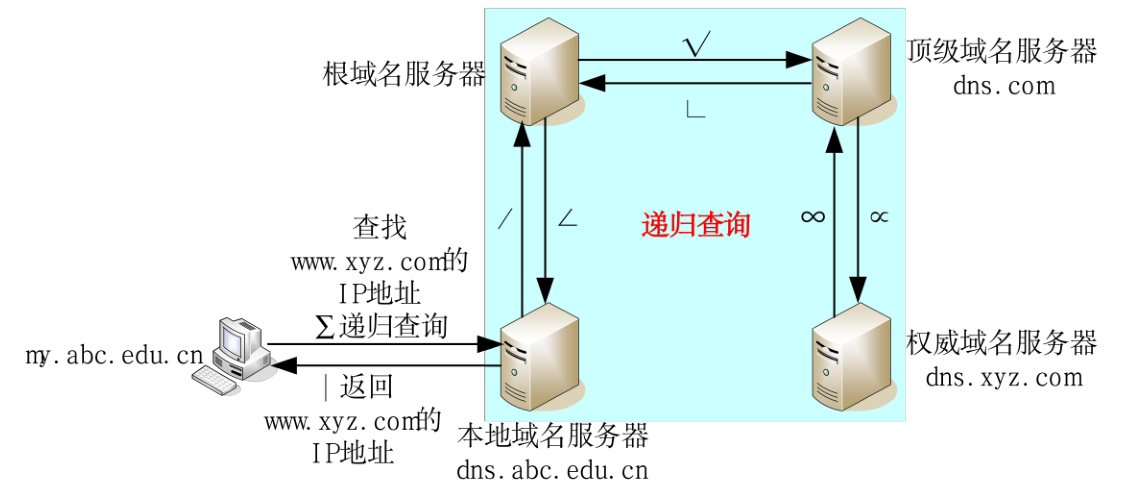
\includegraphics[width=.94\textwidth]{ch06-dns-recursive.png}
\caption{课件上半图：根服务器接手递归解析，并沿层级查询后把结果返回本地服务器，再答复主机。箭头表示查询或结果返回方向。来源：\texttt{Chapter6-应用层.pdf}，PDF第27页（显示页27），局部截取。}
\end{figure}
\begin{figure}[H]\centering
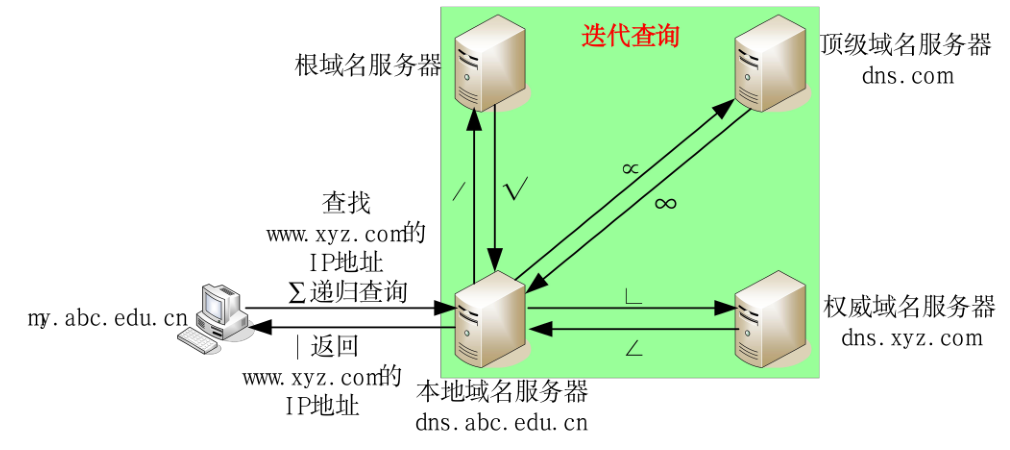
\includegraphics[width=.80\textwidth]{ch06-dns-iterative.png}
\caption{课件下半图：本地DNS服务器依次询问根、TLD和权威服务器；每次转介后，本地服务器自己向下一层查询。来源：\texttt{Chapter6-应用层.pdf}，PDF第27页（显示页27），局部截取。}
\end{figure}

\subsection{一次完整的域名解析}
以查询\texttt{www.amazon.com}为例，且假设主机和本地DNS服务器都没有可用缓存：
\begin{enumerate}[nosep]
\item 主机向本地DNS服务器发送查询请求；主机把后续查询委托给本地DNS服务器。
\item 本地DNS服务器先查自己的缓存。若未命中，它向根服务器发出迭代查询。
\item 根服务器返回\texttt{com}顶级域服务器的信息。本地DNS服务器据此向TLD服务器查询。
\item TLD服务器返回负责\texttt{amazon.com}的权威服务器信息；本地DNS服务器再向该权威服务器查询。
\item 权威服务器返回\texttt{www.amazon.com}对应的地址记录。本地DNS服务器缓存结果，并把答案交还主机。
\end{enumerate}

\textbf{课件例题（PDF第33页）。} 本地DNS服务器无缓存，使用递归方式解析另一个网络中的主机名，问主机与本地DNS服务器分别发几条查询消息？\textbf{解：}主机只向本地DNS服务器发起一次查询；本地DNS服务器作为代理发起后续递归解析。无缓存时主机和本地DNS服务器各自都发送一条查询，因此选A“一条、一条”。如果改成本地DNS服务器对外采用迭代方式，本地服务器会分别询问根、TLD和权威服务器，外部查询消息数就会多于一条；主机仍只需问本地服务器一次。

DNS记录会被服务器缓存一段时间，过期后删除。记录的\textbf{生存时间（Time To Live，TTL）}给出缓存有效期；缓存减少后续查询流量和等待时间，但也意味着记录更新后旧答案可能在TTL到期前继续被使用。

\subsection{资源记录与DNS消息}
DNS数据库中的一条记录称为\textbf{资源记录（Resource Record，RR）}，课件用\texttt{(name, value, type, ttl)}表示。常见类型如下：
\begin{center}\begin{tabularx}{.96\textwidth}{lXX}\toprule
类型 & Name & Value \\\midrule
A & 主机域名 & IPv4地址 \\
NS & 域名 & 该域权威域名服务器的主机名 \\
CNAME & 别名 & 对应的真实域名 \\
MX & 域名 & 为该域接收邮件的邮件服务器名 \\\bottomrule\end{tabularx}\end{center}

\textbf{注册域名的课件例。} 注册\texttt{networkutopia.com}时，注册机构把该域的NS记录以及权威服务器的A记录加入\texttt{com}的DNS信息；随后在权威服务器中为Web主机配置A记录，并为邮件服务器配置MX记录和对应的A记录。邮件地址中的主机部分由MX记录指向邮件服务器，不能把MX记录误认为邮件服务器IP地址。\textbf{课件记号提示：}第32页上方写\texttt{networkutopia.com}，后续示例中又出现\texttt{networkuptopia.com}（多出一个字母\texttt{p}）；本笔记沿用上方域名，只讲解记录配置关系，不据拼写差异推断两个域名的关系。

DNS查询与回复使用相同格式的消息。课件给出的固定首部长度为12字节，包含六组字段：16位消息标识、标志位、问题数、回答资源记录数、权威资源记录数和附加资源记录数。消息标识字段是16位编号，回复复制该编号，使请求方能匹配查询与回答。标志位说明这是查询还是回复、是否期望递归、服务器是否支持递归以及回答是否权威。首部之后依次是问题、回答、权威记录和附加信息四个部分；问题部分列出要查询的Name与Type，回答部分给出资源记录，权威部分可列出权威服务器信息，附加部分可放置帮助后续查询的信息。

\textbf{参考书补充：}DNS通常使用UDP承载查询，服务器端使用熟知端口53；若查询内容较大或响应需要可靠传输，也可能使用TCP。课件示例重点在命名层级和查询过程，没有展开这些传输层细节。

\annotationarea[4]
\small 来源：\texttt{Chapter6-应用层.pdf}，PDF阅读器第20--33页（显示页20--33）；参考书PDF第281--287页（印刷第270--276页）。课件第27页两幅查询图分别局部裁取；第33页递归查询选择题已逐步解答。\normalsize

\section{文件传输协议FTP}
\subsection{控制连接与数据连接}
\textbf{文件传输协议（File Transfer Protocol，FTP）}使用客户/服务器结构，在TCP上提供远程文件浏览、上传与下载。客户端先连接FTP服务器的TCP端口21，建立\textbf{控制连接}；用户名、密码、目录操作和传输命令经此连接发送。控制连接在整个FTP会话期间保持打开，文件内容不通过该连接传送。

服务器收到传输命令后，再为文件或目录列表建立\textbf{数据连接}。数据传输结束后数据连接关闭；若还要传另一个文件，可重新建立数据连接。控制命令与文件内容分开传输称为带外控制。课件图中的端口20是经典主动模式示例。

\begin{figure}[H]\centering
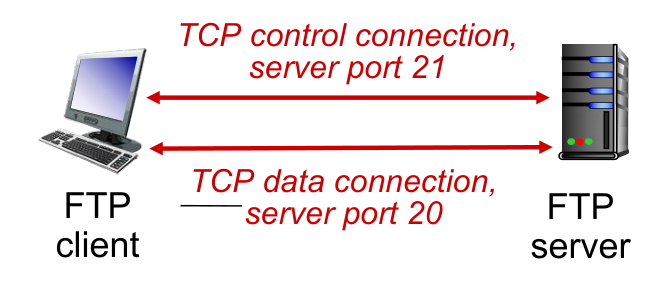
\includegraphics[width=.72\textwidth]{ch06-ftp-connections.png}
\caption{FTP将端口21上的控制连接与文件数据连接分开；课件图中数据连接的服务器端口20对应主动模式示意。来源：\texttt{Chapter6-应用层.pdf}，PDF第36页（显示页36），局部截取。}
\end{figure}

\textbf{参考书补充：}主动（PORT）模式下，服务器从自己的20号端口主动连到客户端提供的端口；被动（PASV）模式下，服务器告知客户端一个临时数据端口，由客户端主动连接。因此，端口20不是所有FTP数据连接都必然使用的端口。两种方式下控制连接都在服务器21号端口，客户端控制连接端口通常由系统分配。

\subsection{FTP命令与逐事件例子}
课件列出的控制命令以ASCII文本发送：\texttt{USER username}提交用户名，\texttt{PASS password}提交密码，\texttt{LIST}列出当前目录，\texttt{RETR filename}下载文件，\texttt{STOR filename}上传文件。服务器用状态码和文字回应，例如\texttt{331}表示用户名已收到、需要密码；\texttt{125}表示数据连接已打开、传输将开始；\texttt{425}表示无法打开数据连接；\texttt{452}表示写文件出错。

\textbf{下载事件例。}客户端连接服务器TCP 21号端口，随后通过控制连接发送登录信息；服务器验证成功后，客户端浏览目录并发送\texttt{RETR report.pdf}；服务器按当前传输模式建立数据连接；文件字节通过数据连接发送；文件传完后数据连接关闭，控制连接仍可继续用来下载另一个文件。\texttt{LIST}返回的目录列表也通过数据连接传输。

\annotationarea[4]
\small 来源：\texttt{Chapter6-应用层.pdf}，PDF阅读器第35--37页（显示页35--37）；参考书PDF第287--293页（印刷第276--282页）。主动/被动模式为参考书对课件双连接机制的补充。\normalsize

\section{电子邮件}
\subsection{系统组成与邮件投递}
电子邮件是一种异步通信方式：收件人不必与发件人同时在线。\textbf{用户代理（User Agent，UA）}是邮件客户端，用于撰写、发送、接收和管理邮件；\textbf{邮件服务器}负责接收邮件、暂存待发送邮件，并把来信放入收件人的邮箱。\textbf{简单邮件传输协议（Simple Mail Transfer Protocol，SMTP）}用于发送邮件及邮件服务器之间的投递；\textbf{邮局协议第3版（Post Office Protocol version 3，POP3）}、\textbf{互联网报文存取协议（Internet Message Access Protocol，IMAP）}或Web页面使用的HTTP可用于用户读取邮件。

\begin{figure}[H]\centering
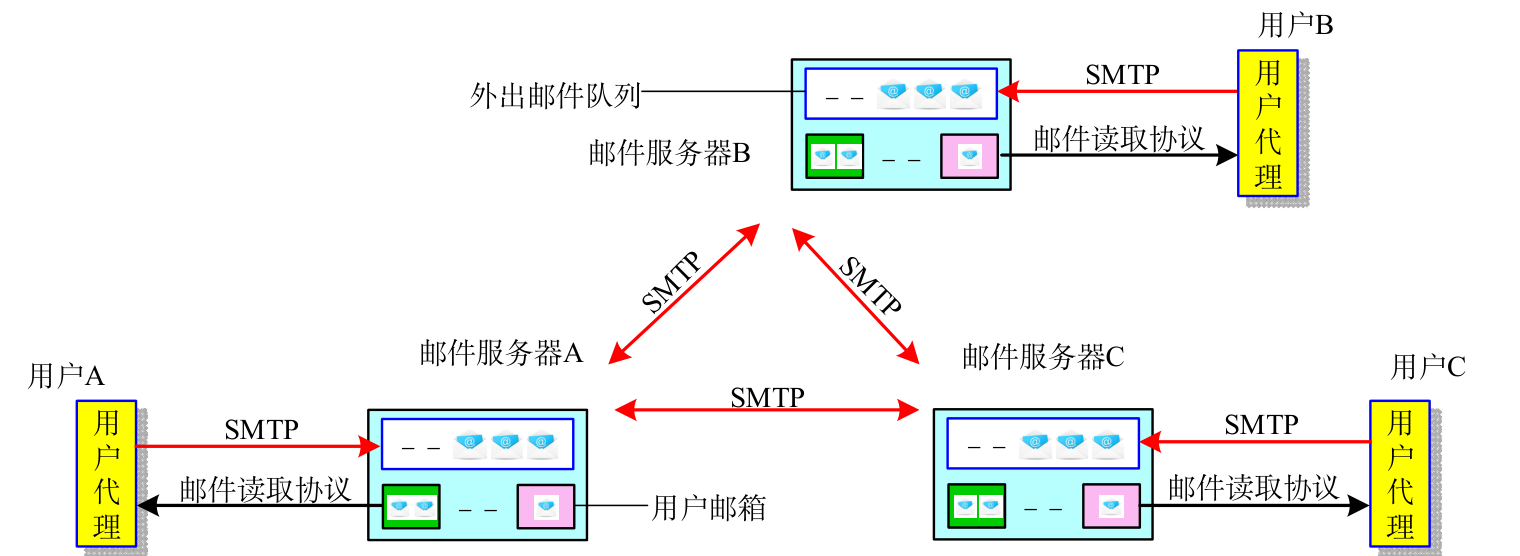
\includegraphics[width=.96\textwidth]{ch06-email-system.png}
\caption{邮件客户端把邮件交给邮件服务器；邮件服务器之间用SMTP投递，收件人通过邮件读取协议访问邮箱。箭头表示协议方向。来源：\texttt{Chapter6-应用层.pdf}，PDF第39页（显示页39），局部截取。}
\end{figure}

一次常见邮件流程为：发件人用用户代理撰写邮件并提交给发送端邮件服务器；邮件服务器把邮件放入外出队列；发送端服务器作为SMTP客户连接接收端邮件服务器并发送邮件；接收端服务器把邮件存入收件人邮箱；收件人之后通过POP3、IMAP或Web邮件读取。邮件服务器既能作为SMTP服务器接收邮件，也能作为SMTP客户向下一台邮件服务器发送邮件。

\subsection{SMTP及消息格式}
\textbf{简单邮件传输协议（Simple Mail Transfer Protocol，SMTP）}通过TCP可靠发送邮件，服务器端熟知端口为25。SMTP采用命令/响应方式，课件按握手、传输、关闭三个阶段说明。典型会话如下：

\begin{quote}\small\ttfamily
S: 220 hamburger.edu\\
C: HELO crepes.fr\\
S: 250 Hello crepes.fr, pleased to meet you\\
C: MAIL FROM: <alice@crepes.fr>\\
S: 250 Sender ok\\
C: RCPT TO: <bob@hamburger.edu>\\
S: 250 Recipient ok\\
C: DATA\\
S: 354 End mail with a line containing only a period\\
C: Do you like ketchup?\\
C: How about pickles?\\
C: .\\
S: 250 Message accepted for delivery\\
C: QUIT\\
S: 221 Closing connection
\end{quote}

读这段交互时，\texttt{C}是当前SMTP客户，\texttt{S}是服务器。\texttt{HELO}标识客户端；\texttt{MAIL FROM}给出发件人；\texttt{RCPT TO}指定收件人；\texttt{DATA}后开始传邮件内容；只含一个句点的行结束邮件内容；\texttt{QUIT}请求关闭会话。这里的客户端可以是用户代理，也可以是发送端邮件服务器。

SMTP连接通常在一次邮件传送会话中保持打开。课件所述基础SMTP邮件正文使用7位ASCII字符；HTTP与SMTP都使用可读文本命令和状态码，但方向和消息组织不同：HTTP通常由客户拉取对象，SMTP由发送方把邮件推送到接收方；HTTP的多个对象通常分别响应，邮件内容可由多个部分组成。

邮件内容有首部和主体，中间以空行分隔。常见首部行包括\texttt{From}、\texttt{To}和\texttt{Subject}；主体是邮件正文。课件的示例格式如下：
\begin{quote}\small\ttfamily
From: alice@crepes.fr\\
To: bob@hamburger.edu\\
Subject: Picture of yummy crepe.\\
\\
邮件正文……
\end{quote}

\textbf{MIME（Multipurpose Internet Mail Extensions，多用途互联网邮件扩展）}让邮件可以表示非ASCII文本和图像等多媒体内容。它通过邮件首部说明内容类型与编码方式，例如：
\begin{quote}\small\ttfamily
Content-Type: image/jpeg\\
Content-Transfer-Encoding: base64
\end{quote}
编码后的内容仍可经基础邮件传输方式传送。MIME扩展邮件格式和编码，不取代SMTP。课件第45页把MIME相关RFC写为“2045、2056”。其中RFC 2056的标题是“Uniform Resource Locators for Z39.50”，MIME Part Two对应RFC 2046；结合参考书在本节引用RFC 2045，可确认课件此处应为“2045、2046”，将“2056”订正为“2046”（\href{https://www.rfc-editor.org/info/rfc2046/}{RFC 2046}）。

\subsection{邮件读取：POP3与IMAP}
\textbf{邮局协议第3版（Post Office Protocol version 3，POP3）}用于用户代理从邮件服务器读取邮件。用户先用\texttt{USER}和\texttt{PASS}完成认证，服务器以\texttt{+OK}或\texttt{-ERR}回应；用户随后可用\texttt{LIST}列出邮件、\texttt{RETR}取回邮件、\texttt{DELE}标记删除，最后用\texttt{QUIT}结束会话。POP3可采用“下载并删除”或“下载并保留”的方式。按课件的基本模型，POP3不在服务器维护跨会话的文件夹状态。

\textbf{互联网报文存取协议（Internet Message Access Protocol，IMAP）}通常把邮件留在服务器上，支持用文件夹组织邮件，并保存跨会话的文件夹名、邮件与文件夹对应关系等状态。相较之下，POP3规则简单、功能较少。通过浏览器使用Web邮箱时，浏览器与邮件服务之间可用HTTP交互。

\textbf{POP3逐事件例。}用户代理发送\texttt{USER bob}，服务器以\texttt{+OK}回应；代理发送\texttt{PASS}，验证成功后用\texttt{LIST}获取邮件编号和大小；发送\texttt{RETR 1}读取1号邮件；若采用下载并删除方式，再发\texttt{DELE 1}；最后发\texttt{QUIT}关闭会话。若选下载并保留，读取后不删除服务器副本。

\annotationarea[4]
\small 来源：\texttt{Chapter6-应用层.pdf}，PDF阅读器第39--49页（显示页39--49）；参考书PDF第294--300页（印刷第283--289页）。课件第45页的RFC编号已按RFC 2046订正并附来源。\normalsize

\section{万维网与HTTP}
\subsection{Web对象、URL与HTTP交互}
\textbf{万维网（World Wide Web，WWW）}由相互链接的网页和网页对象构成。网页中的对象可以是\textbf{超文本标记语言（HyperText Markup Language，HTML）}文件、图片、视频或脚本等。\textbf{统一资源定位符（Uniform Resource Locator，URL）}标识资源的位置和访问方式，课件给出的一般形式为
\[
\texttt{scheme://host:port/path}.
\]
其中scheme表示访问资源的协议，host是服务器域名或IP地址，port是服务器端口，path指出主机上的资源位置；若端口省略，则使用协议约定的默认值。URL例子\url{www.someschool.edu/someDept/pic.gif}中，前半部分是主机名，后半部分是路径。

\textbf{超文本传输协议（HyperText Transfer Protocol，HTTP）}是浏览器和Web服务器交换请求、响应的应用层协议。课件基础模型中，浏览器先建立到服务器TCP 80端口的连接，再经连接发送HTTP请求并接收响应。HTTP协议本身是\textbf{无状态}的：服务器不因一次请求而自动记住同一客户以前请求过什么。底层TCP提供可靠字节流，但不意味着HTTP有固定响应时限。

\subsection{HTTP请求与响应消息}
HTTP消息采用文本形式。请求消息由请求行、若干首部行、空行和可选消息体组成。请求行包含方法、资源路径和协议版本；首部行传递主机名、连接方式、浏览器类型或语言偏好等信息。课件示例：
\begin{quote}\small\ttfamily
GET /somedir/page.html HTTP/1.1\\
Host: www.someschool.edu\\
User-agent: Mozilla/4.0\\
Connection: close\\
Accept-language: fr\\
\\
\end{quote}
首行表示获取资源；空行表示请求首部结束。响应消息由状态行、首部行、空行和可选消息体组成：
\begin{quote}\small\ttfamily
HTTP/1.1 200 OK\\
Connection: close\\
Date: Thu, 06 Aug 1998 12:00:15 GMT\\
Server: Apache/1.3.0 (Unix)\\
Last-Modified: Mon, 22 Jun 1998\\
Content-Length: 6821\\
Content-Type: text/html\\
\\
……请求的HTML对象……
\end{quote}

常用请求方法：\texttt{GET}取回对象；\texttt{POST}把用户表单等内容放在消息体中提交；\texttt{HEAD}请求首部而不取回对象主体；\texttt{PUT}把消息体中的对象存入指定URL；\texttt{DELETE}删除指定URL标识的对象。使用GET提交表单时，输入可编码到URL的查询部分，例如\texttt{/animalsearch?monkeys\&banana}；POST则把输入放在请求消息体中。

响应状态码在状态行中，课件示例包括：\texttt{200 OK}表示请求成功；\texttt{301 Moved Permanently}表示资源已永久移动；\texttt{400 Bad Request}表示请求有误；\texttt{404 Not Found}表示未找到资源；\texttt{505 HTTP Version Not Supported}表示服务器不支持所请求的HTTP版本。响应首部中的\texttt{Content-Length}表示主体长度，\texttt{Content-Type}说明主体类型。

\subsection{连接方式和HTTP响应时间}
\textbf{非持久连接}中，一个TCP连接传输一个对象；HTTP/1.0课件模型采用这种方式。若HTML页面引用图片，每个对象都需另建TCP连接。\textbf{持久连接}中，服务器发送完响应后保持TCP连接打开，后续请求和对象可复用该连接；HTTP/1.1课件模型默认采用持久连接。

\textbf{往返时间（Round-Trip Time，RTT）}是一个小分组从客户端到服务器并返回所经历的时间。为解释课件的时延公式，作如下假设：忽略DNS解析、排队、处理和小请求的发送时长，TCP按课件图的方式建立连接，服务器收到HTTP请求后开始返回对象。
\begin{itemize}[nosep]
\item 请求一个对象的非持久连接响应时间约为$2\mathrm{RTT}+t_{\mathrm{obj}}$：一个RTT用于建立TCP连接，另一个RTT用于发送请求并等到响应开始到达，$t_{\mathrm{obj}}$是对象传输时间。
\item 非流水持久连接只建立一次TCP连接，但客户必须等上一个对象响应后才请求下一个对象。若网页含基本HTML对象和$k$个引用对象，理想化总时间约为$\mathrm{RTT}+(k+1)\mathrm{RTT}+\sum t_i=(k+2)\mathrm{RTT}+\sum t_i$。
\item 流水持久连接允许客户尽快连续发出多个请求。在课件的理想模型中，基本HTML对象先需约$2\mathrm{RTT}$；解析HTML后，对引用对象的请求与响应可在约$1\mathrm{RTT}$内完成，再加对象传输时间。
\item 浏览器也可并行打开多个非持久TCP连接，使多个引用对象同时传输；并行能缩短对象组的等待时间，但增加连接和服务器资源开销。
\end{itemize}

\textbf{按课件公式计算的例子。} 若RTT为80 ms，对象大小为2 Mbit，瓶颈传输速率为10 Mbit/s，则对象传输时间为$2/10=0.2$ s。忽略其他延迟，单对象非持久连接响应时间约为$2\times0.08+0.2=0.36$ s。

\begin{figure}[H]\centering
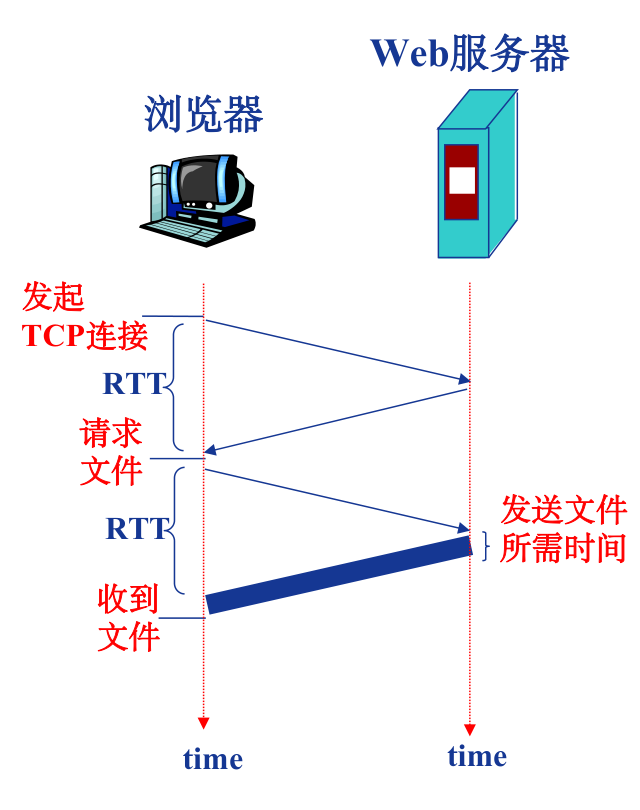
\includegraphics[width=.46\textwidth]{ch06-http-timing.png}
\caption{HTTP/1.0单对象时间线：第一段RTT建立TCP连接，第二段RTT发送请求并等响应开始到达，深色斜条表示对象传输时间。来源：\texttt{Chapter6-应用层.pdf}，PDF第63页（显示页63），局部截取。}
\end{figure}

\textbf{HTTP/1.1流水与队头阻塞。}非流水方式中，收到一个响应后才发下一个请求；流水方式中，发现引用对象后即可连续发送请求。HTTP/1.1按序在一个TCP字节流上传输数据。如果前面的大对象排在小对象之前，小对象会等待；若TCP遇到丢包恢复，后续字节也要等缺失数据补齐。这种等待称为\textbf{队头阻塞（Head-of-Line blocking，HOL blocking）}。

\textbf{HTTP/2与HTTP/3。}课件说明HTTP/2把对象拆成帧，让不同对象的帧交替传输，并可按客户指定的优先级安排对象；课件也提到服务器推送客户尚未请求的对象。交错帧减少对象排队造成的应用层阻塞，但若共享TCP连接丢包，TCP仍要按序交付数据，仍可能暂停多个对象。HTTP/3采用QUIC（Quick UDP Internet Connections）承载HTTP：QUIC运行在UDP之上，在应用层实现可靠性、拥塞控制、连接建立和加密相关功能，并让多个应用级流共享连接。课件强调，一个流的数据丢失不必阻塞其他流继续交付，因而可避免跨流的TCP队头阻塞。

课件第73页把QUIC建立连接标成“1轮握手”，并与单独进行TCP和TLS握手的“2轮”作对比。这是课件用于解释减少建立时延的示意；实际握手时延会依协议版本、连接状态和实现条件而变，计算题应按题目给定条件使用。

\subsection{代理缓存、条件GET与Cookie}
\textbf{Web缓存/代理服务器（Web cache/proxy）}保存近期访问的对象。浏览器把HTTP请求发给代理：若缓存命中，代理直接把对象返回，代理此时作为服务器；若未命中，代理作为客户向原始服务器请求对象，取得后返回浏览器并保存副本。缓存靠近用户时可减少访问时延，也能降低组织出口链路流量。

\begin{figure}[H]\centering
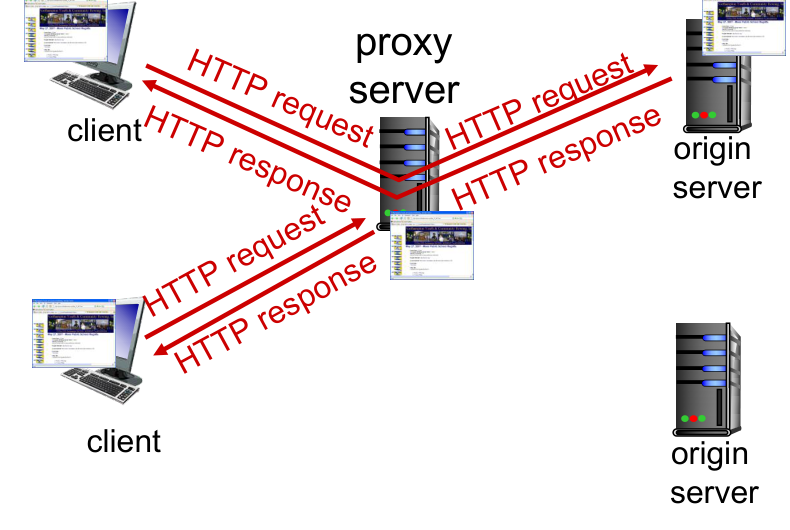
\includegraphics[width=.80\textwidth]{ch06-web-cache.png}
\caption{Web缓存同时面对客户端和原始服务器：命中时从代理直接返回，未命中时由代理请求源站并把对象缓存。箭头表示HTTP请求或响应方向。来源：\texttt{Chapter6-应用层.pdf}，PDF第77页（显示页77），局部截取。}
\end{figure}

\textbf{课件缓存计算例（PDF第79--81页）。} 假定对象平均大小$F=1$ Mbit，每秒向原始服务器请求$\lambda=10$个对象，机构出口速率$R=10$ Mbit/s，客户端到原始服务器RTT为2 s。出口链路提供的平均数据率为$\lambda F=10$ Mbit/s，因此链路利用率$\rho=\lambda F/R=1$，排队延迟会很大；\textbf{局域网（Local Area Network，LAN）}为1 Gbit/s，其平均利用率约为$10/1000=1\%$。把出口链路升到100 Mbit/s后，利用率降到10\%，课件估计链路排队延迟降为几毫秒，局域网延迟为几微秒；总延迟仍约为2 s加上这两项。扩容可改善访问等待，但课件指出成本较高。

若改用本地缓存，命中率为0.4，则40\%的请求本地返回，只有60\%到源服务器。出口平均流量变为$0.6\lambda F=6$ Mbit/s，10 Mbit/s链路利用率约60\%。按课件假设，未命中请求的主要往返延迟为2 s，本地命中只需数微秒，因此平均响应时间约为
\[
0.6\times 2\,\mathrm{s}+0.4\times(\text{数微秒})\approx1.2\,\mathrm{s}.
\]
计算时，先用命中率求需要访问源站的比例，再按命中与未命中的等待时间加权。注意这只是课件给出的平均值估算；没有把链路排队模型的全部参数逐项展开。

\textbf{条件性GET（conditional GET）}帮助代理确认缓存对象是否仍是最新版本。代理在请求中发送\texttt{If-Modified-Since: <date>}；若服务器确认对象未变化，则返回\texttt{304 Not Modified}且不重传对象；若对象已变化，则返回\texttt{200 OK}及新对象。

\textbf{Cookie}用于在无状态HTTP之上关联同一浏览器的多次访问。首次访问时，服务器在响应中发送\texttt{Set-Cookie: 1678}并在后台数据库创建对应记录；浏览器把Cookie保存在本地，之后访问同一站点时在请求中发送\texttt{Cookie: 1678}，服务器据此找到用户状态并提供购物车、登录或推荐等服务。Cookie有利于会话管理，但也带来隐私问题。

\begin{figure}[H]\centering
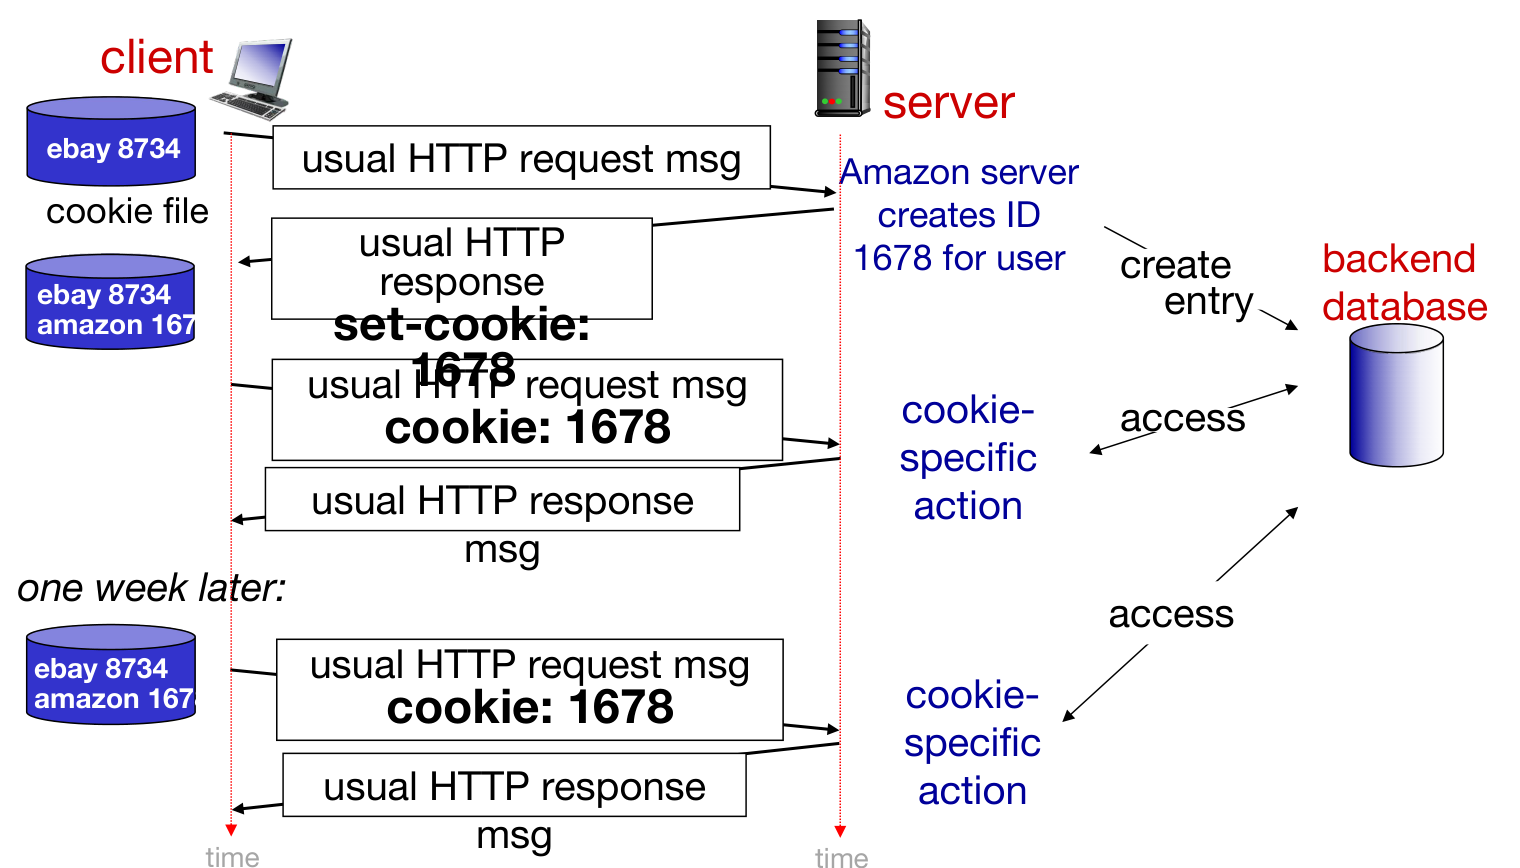
\includegraphics[width=.92\textwidth]{ch06-cookie.png}
\caption{Cookie事件顺序：服务器首次分配标识并写入后台记录，浏览器保存标识，后续请求带回Cookie供服务器查找状态。来源：\texttt{Chapter6-应用层.pdf}，PDF第86页（显示页86），局部截取。}
\end{figure}

\annotationarea[4]
\small 来源：\texttt{Chapter6-应用层.pdf}，PDF阅读器第51--87页（显示页51--87）；参考书PDF第300--313页（印刷第289--302页）。课件缓存算例与RTT公式均在正文列出假设并给出计算过程。\normalsize

\section{P2P应用与文件分发}
\subsection{客户机/服务器与P2P分发时间}
设文件大小为$F$ bit，要分发给$N$个节点。服务器上传速率为$u_s$ bit/s，第$i$个节点上传速率为$u_i$，下载速率为$d_i$，最慢下载速率为$d_{\min}=\min_i d_i$。分发时间至少要满足文件数据能够从发送端上传、每个节点能下载完整文件这两个基本条件。

\textbf{客户机/服务器分发。}服务器至少要上传$N$份文件，共$NF$ bit；最慢客户至少需要$F/d_{\min}$秒下载一份。因此
\[
D_{\mathrm{C/S}}\geq \max\left\{\frac{NF}{u_s},\frac{F}{d_{\min}}\right\}.
\]
当$N$增大时，服务器上传项$NF/u_s$线性增加，服务器可能成为瓶颈。

\textbf{P2P分发。}服务器至少上传一份文件；每个节点仍须下载完整文件；服务器和所有节点合起来至少要上传总计$NF$ bit。因此
\[
D_{\mathrm{P2P}}\geq \max\left\{\frac{F}{u_s},\frac{F}{d_{\min}},
\frac{NF}{u_s+\sum_{i=1}^{N}u_i}\right\}.
\]
第三项体现P2P节点可以贡献上传能力。这里是理论下界；实际完成时间还受节点在线情况、带宽共享和协议调度等因素影响。

\textbf{课件参数例（PDF第93页）。}设每个节点上传速率为$u$，服务器上传速率$u_s=10u$，最慢下载速率$d_{\min}\geq u_s$，且$F/u=1$小时。取$N=100$：
\[
D_{\mathrm{C/S}}\geq\max\{100F/(10u),F/d_{\min}\}=\max\{10,\leq0.1\}\text{小时}=10\text{小时}.
\]
P2P下$\sum_i u_i=100u$，所以
\[
D_{\mathrm{P2P}}\geq\max\left\{0.1,\leq0.1,\frac{100F}{110u}\right\}
\text{小时}\approx0.91\text{小时}.
\]
两式是下界比较，说明当用户多、对等节点能贡献上传时，P2P不必像C/S那样由一个服务器承担全部副本；它不保证任意网络实际用时都恰好等于该下界。

\subsection{BitTorrent文件交换}
课件用\textbf{BitTorrent}说明P2P文件交换。一个文件被切成固定大小的块（chunk），课件示例大小为256 KB；正在交换同一文件块的一组节点称为一个\textbf{torrent}。\textbf{Tracker}记录参与torrent的节点，帮助新节点取得邻居列表，但实际文件块在peer之间交换。

\begin{figure}[H]\centering
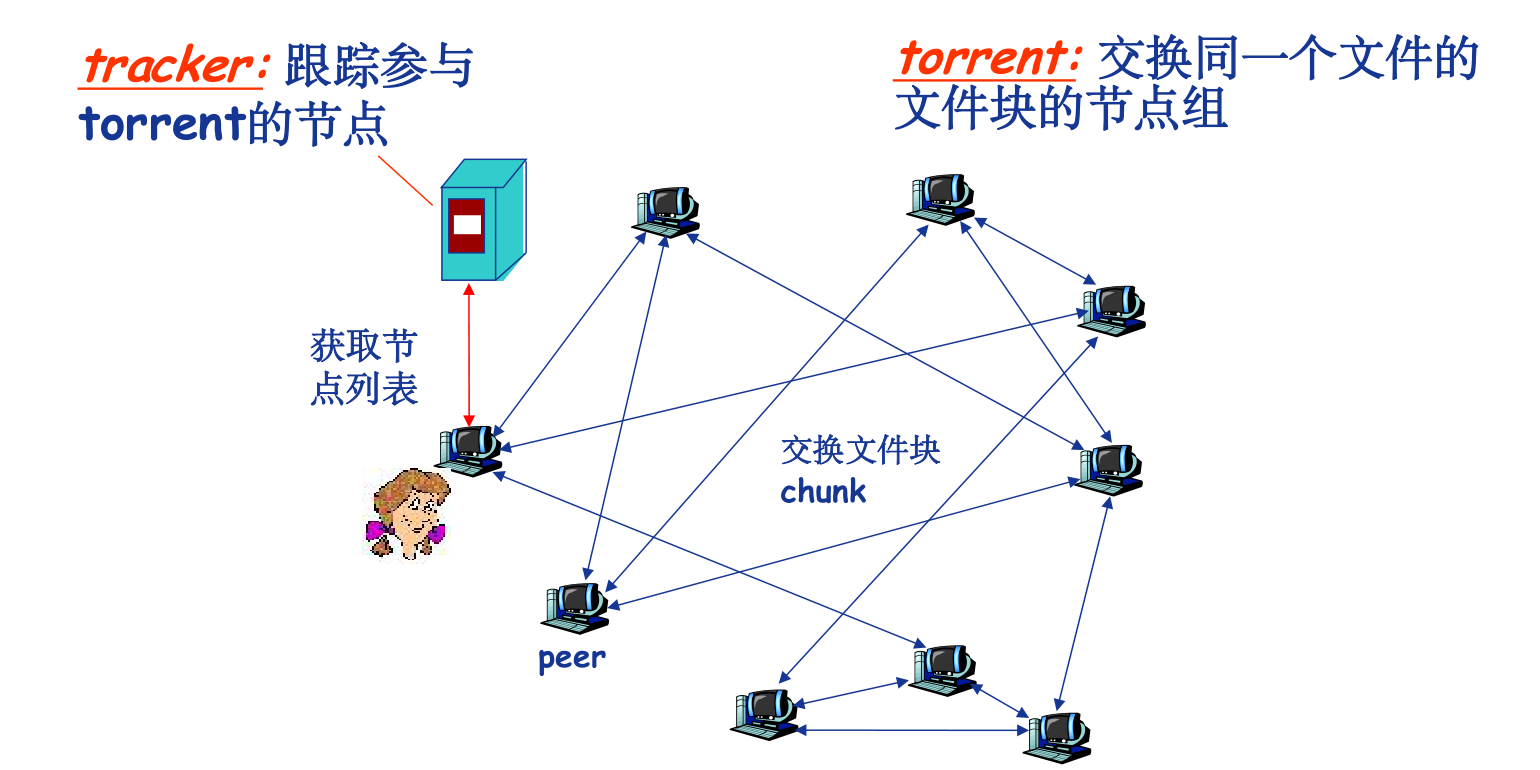
\includegraphics[width=.86\textwidth]{ch06-bittorrent.png}
\caption{Tracker帮助新peer取得参与节点列表；蓝色箭头表示peer之间交换文件块，而非经Tracker中转。来源：\texttt{Chapter6-应用层.pdf}，PDF第94页（显示页94），局部截取。}
\end{figure}

新节点加入时还没有文件块，先向Tracker登记并取得节点清单，再连接其中一些邻居。节点下载的同时也向其他节点上传；节点可以加入或离开。节点定期查询邻居持有的块列表，并向邻居请求自己缺少的块。课件列出的\textbf{稀缺优先（rarest first）}原则是优先请求当前较少见的块，避免稀有块只留在少数节点上。

\textbf{Tit-for-tat（以牙还牙）}用上传合作鼓励互惠：Alice优先向当前给她较快上传的4个邻居提供块，并每10秒重新评估；此外每30秒随机选一个其他节点试传块，这称为\textbf{乐观解封（optimistic unchoke）}。随机试传可能发现更好的交换伙伴，双方随后都能进入对方的较快上传邻居集合。节点取得完整文件后可以离开，也可以留下继续上传。

\begin{figure}[H]\centering
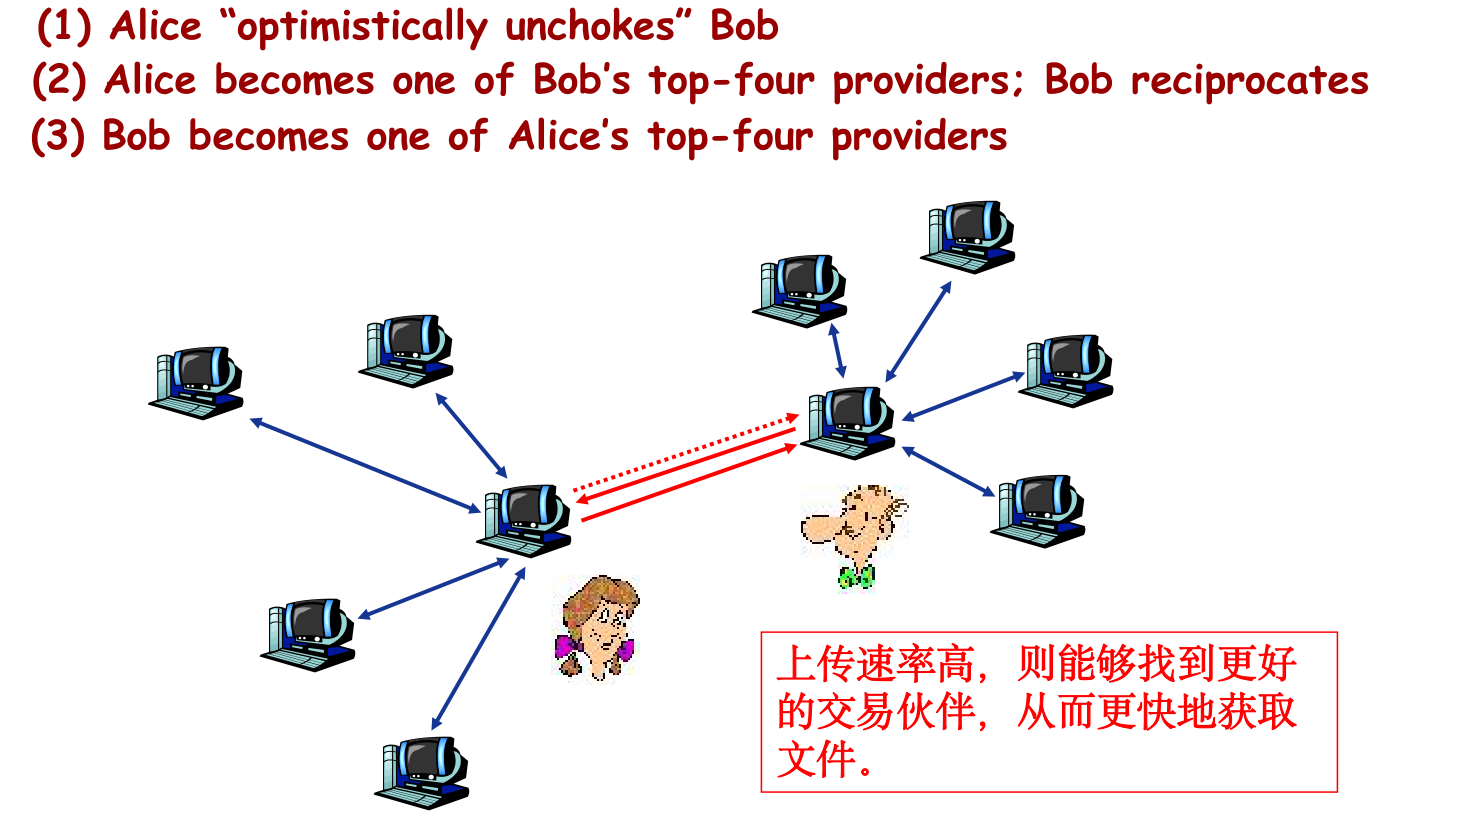
\includegraphics[width=.90\textwidth]{ch06-bittorrent-unchoke.png}
\caption{乐观解封建立新的试传机会；如果互相上传后成为对方较快的前四个提供者，双方会继续互惠。来源：\texttt{Chapter6-应用层.pdf}，PDF第97页（显示页97），局部截取。}
\end{figure}

\subsection{P2P索引与分布式哈希表}
P2P应用还需要解决“内容在哪里”的问题。\textbf{索引}是从内容或用户名映射到节点位置（IP地址与端口号）的信息。课件比较了集中式索引、洪泛式查询、层次式覆盖网络和分布式哈希表。

\begin{itemize}[nosep]
\item \textbf{集中式索引：}Napster中节点加入时向中央目录登记IP地址和共享内容；Alice查询文件名后，目录返回持有文件的节点，Alice再直接向该节点请求文件。目录单点故障或过载会影响查找；内容和文件传输虽分布在节点之间，定位仍集中。
\item \textbf{洪泛式查询（query flooding）：}Gnutella例中，每个节点只索引自己共享的文件；活动节点之间的TCP连接构成覆盖网络（overlay network），其边是逻辑上的虚拟链路。查询沿已有连接向邻居扩散；若某节点命中，就沿查询来路返回QueryHit；随后文件可由节点间传输。洪泛无需中央索引，但可能产生较多查询消息。
\item \textbf{层次式覆盖网络：}部分节点充当超级节点，普通节点连接某个超级节点，超级节点之间也可连接。超级节点跟踪所辖节点的内容，形成介于集中式索引与完全洪泛之间的组织方式。
\item \textbf{分布式哈希表（Distributed Hash Table，DHT）：}把键值对分散存放在众多peer上；查询给出key，系统返回匹配的value，节点也能插入键值对。
\end{itemize}

DHT把原始key通过哈希函数转成整数，并给peer也分配相同范围内的整数标识符。若标识符用$n$ bit表示，范围为$[0,2^n-1]$。课件约定把key分配给\textbf{顺时针方向遇到的第一个peer（successor）}。例如$n=4$、peer标识为$1,3,4,5,8,10,12,14$：key 13由peer 14负责；key 15顺时针绕回后由peer 1负责。

\textbf{环形DHT查找。}若每个peer只知道直接后继和前驱，查询会沿环逐个转发，课件给出的平均消息数为$O(N)$。增加shortcut（快捷连接）后，一个peer可按规则跳到更远节点；课件说明可用$O(\log N)$个邻居把查找消息数降至$O(\log N)$。图中红色箭头表示key 1110从发起peer沿快捷路径转发并交给顺时针后继。

\begin{figure}[H]\centering
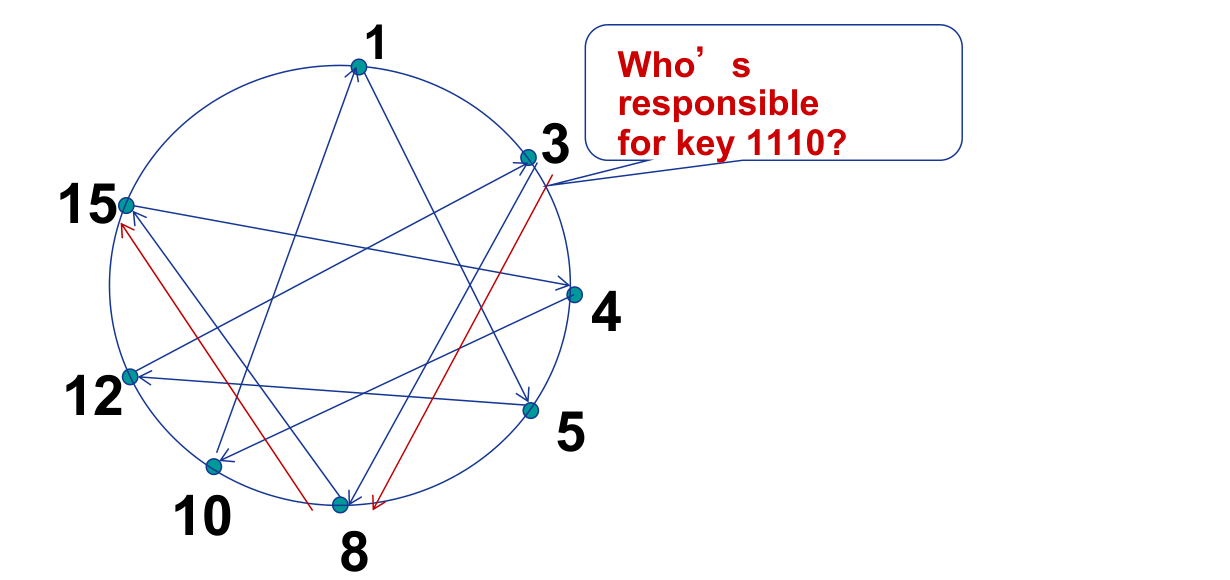
\includegraphics[width=.76\textwidth]{ch06-dht-ring.png}
\caption{环形DHT及快捷连接示意：蓝色边是peer间覆盖连接，红色箭头展示key查询的转发方向；按顺时针后继确定负责该key的peer。来源：\texttt{Chapter6-应用层.pdf}，PDF第111页（显示页111），局部截取。}
\end{figure}

\textbf{节点动态变化（peer churn）。}P2P节点会加入、离开或突然失效。课件示例让每个peer记住两个后继并定期ping它们；若直接后继失效，就把第二后继提升为新的直接后继，再询问它的后继以补足列表。例如peer 5离开后，peer 4把peer 8设为直接后继，并向peer 8询问下一个后继。维护后继列表可降低单个节点失效导致环断裂的风险。

\annotationarea[4]
\small 来源：\texttt{Chapter6-应用层.pdf}，PDF阅读器第89--112页（显示页89--112）。教材PDF第278--280页（印刷第267--269页）核对C/S与P2P模型；文件分发公式、BitTorrent、覆盖网络和DHT按课件整理。\normalsize

\section{Socket API与TCP调用流程}
\subsection{API、套接字描述符与地址}
\textbf{应用编程接口（Application Programming Interface，API）}是应用进程调用操作系统功能的接口。课件用Socket API说明应用程序如何创建通信端点、设置地址、建立TCP连接、发送和接收数据。套接字对外由IP地址和端口标识；对进程内部，操作系统返回一个小整数\textbf{套接字描述符（socket descriptor）}，应用通过它引用套接字。

创建套接字时，操作系统为它保存协议族、服务类型、本地和远端IP及端口等信息。课件给出的IPv4地址结构\texttt{sockaddr\_in}包括地址长度\texttt{sin\_len}、地址族\texttt{sin\_family}（TCP/IP使用\texttt{AF\_INET}）、端口\texttt{sin\_port}、IP地址\texttt{sin\_addr}以及未用字段\texttt{sin\_zero}。不同操作系统的结构定义略有差异，实际编程应以当前平台头文件为准；学习时重点识别地址族、端口和IP地址。

\subsection{常用Socket API函数}
课件以WinSock（Windows Socket Interface）为例。\texttt{WSAStartup}初始化WinSock库，\texttt{WSACleanup}结束使用并释放库资源；它们只用于WinSock。课件示例以\texttt{MAKEWORD(2,1)}请求2.1版，并用\texttt{WSADATA}取得实际版本信息。

\begin{center}\begin{tabularx}{.98\textwidth}{lXX}\toprule
函数 & 作用 & 使用场景 \\\midrule
\texttt{socket} & 创建套接字并返回描述符 & \texttt{PF\_INET}指定IPv4族；\texttt{SOCK\_STREAM}用于TCP，\texttt{SOCK\_DGRAM}用于UDP，\texttt{SOCK\_RAW}为原始套接字 \\
\texttt{bind} & 把本地IP和端口绑定到套接字 & 服务器通常绑定熟知端口；需接收多个本地接口的请求时可用\texttt{INADDR\_ANY} \\
\texttt{listen} & 让流套接字进入监听状态并设连接请求队列大小 & 服务器端TCP套接字 \\
\texttt{connect} & 指定要通信的远端地址 & TCP客户端建立连接；UDP客户端指定默认对端，不进行TCP式握手 \\
\texttt{accept} & 从监听队列取出一个TCP连接请求并返回新的连接套接字 & 服务器端TCP；监听套接字继续接受其他客户 \\
\texttt{send}/\texttt{recv} & 发送/接收字节或数据 & TCP，以及已调用\texttt{connect}的UDP客户端 \\
\texttt{sendto}/\texttt{recvfrom} & 发送/接收数据报并指定/取得对端地址 & 未连接的UDP套接字 \\
\texttt{closesocket} & 关闭或释放套接字描述符 & 使用结束时调用 \\
\texttt{setsockopt}/\texttt{getsockopt} & 设置/读取套接字选项 & 调整或查询套接字行为参数 \\\bottomrule\end{tabularx}\end{center}

服务器通常需要\texttt{bind}到服务端口。多网卡服务器若要在所有IPv4本地接口接收连接，可使用地址通配符\texttt{INADDR\_ANY}。客户端通常无需手动\texttt{bind}，系统可自动选择本地IP和临时端口。TCP服务器的\texttt{listen}负责排队等候请求，\texttt{accept}从队列中取出一个请求，并创建新的连接套接字供该客户使用。

课件给出的\texttt{send}、\texttt{recv}等函数原型是说明参数角色的示意形式，不是适用于所有系统的完整可编译签名。TCP是字节流，接收一次数据不一定与对方一次发送的边界一一对应；UDP则按数据报接收，并通过\texttt{sendto}/\texttt{recvfrom}携带对端地址。

\subsection{TCP客户端与服务器的调用次序}
\begin{figure}[H]\centering
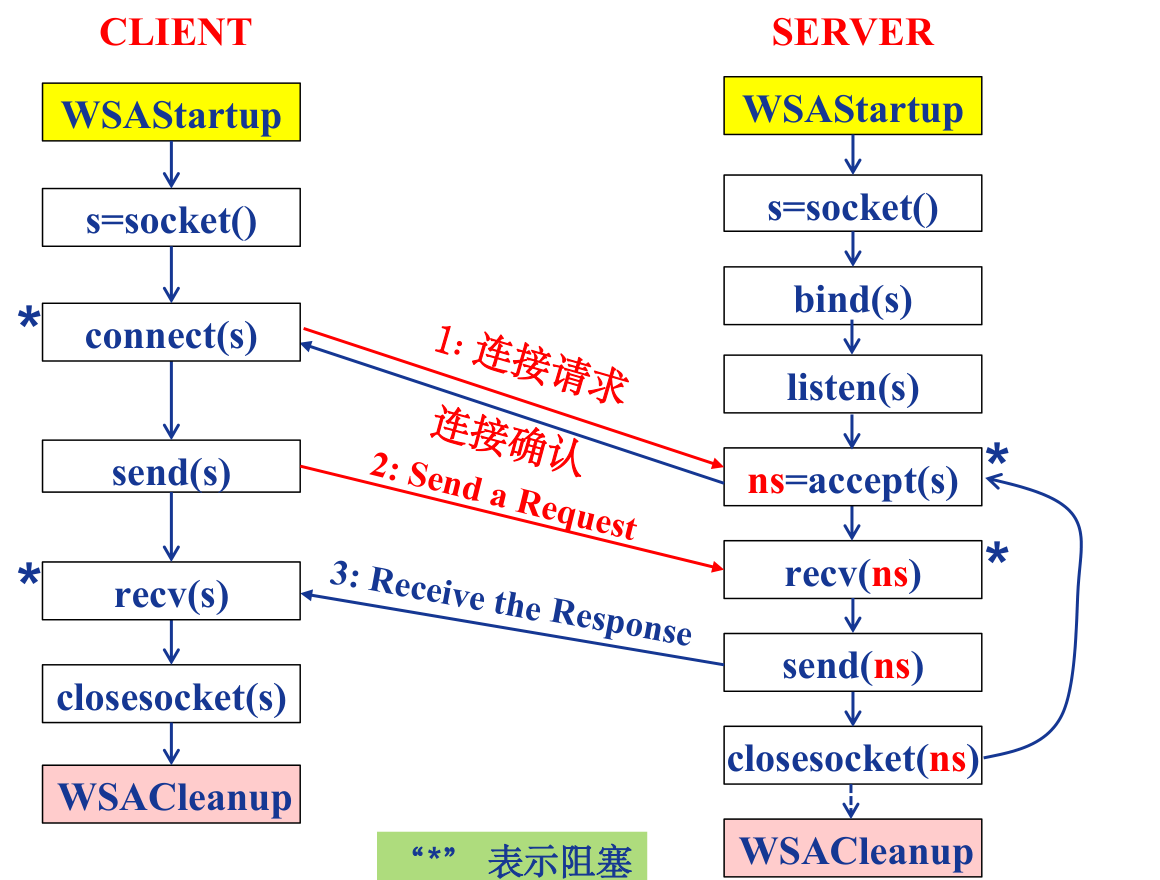
\includegraphics[width=.88\textwidth,height=.68\textheight,keepaspectratio]{ch06-socket-flow.png}
\caption{WinSock TCP基本调用流程：服务器创建、绑定并监听，\texttt{accept}等待连接；客户端\texttt{connect}发起连接后发送请求、接收响应。星号表示可能阻塞等待。来源：\texttt{Chapter6-应用层.pdf}，PDF第137页（显示页137），局部截取。}
\end{figure}

按图读一次请求/响应：
\begin{enumerate}[nosep]
\item 客户端和服务器先分别调用\texttt{WSAStartup}，再各自用\texttt{socket}创建套接字。
\item 服务器用\texttt{bind}绑定服务地址和端口，用\texttt{listen}进入监听，再调用\texttt{accept}等待客户；\texttt{accept}返回新的套接字\texttt{ns}。
\item 客户端调用\texttt{connect}连接服务器；服务器收到请求后，\texttt{accept}解除阻塞并返回\texttt{ns}。
\item 客户端通过\texttt{send}发送请求，服务器在\texttt{recv(ns)}取得数据，处理后用\texttt{send(ns)}返回响应。
\item 客户端用\texttt{recv}接收响应；双方分别用\texttt{closesocket}关闭各自连接端点，最后调用\texttt{WSACleanup}。
\end{enumerate}

图中的监听套接字与连接套接字用途不同：监听套接字负责等待更多连接；\texttt{accept}产生的连接套接字负责和某一个客户交换数据。标有星号的\texttt{connect}、\texttt{accept}、\texttt{recv}可能在条件未满足时阻塞等待。

\subsection{网络字节顺序}
网络协议首部中的多字节整数使用统一的\textbf{网络字节顺序（network byte order）}表示。主机内部的本地字节顺序可能不同，向Socket API传递端口或IP数值前后需转换：\texttt{htons}把16位本地值转成网络顺序，\texttt{ntohs}反向转换；\texttt{htonl}和\texttt{ntohl}分别处理32位值。端口号是16位，IPv4地址是32位。

\textbf{Socket API基础调用练习。}假设服务器TCP端口为80，客户端要发送一次HTTP请求。服务器先创建流套接字、绑定80号端口并监听；客户端创建流套接字并\texttt{connect}服务器IP与80号端口；服务器\texttt{accept}并取得专用连接套接字；客户端\texttt{send}请求，服务器\texttt{recv}请求并\texttt{send}响应，客户端\texttt{recv}响应；最后双方关闭连接套接字。注意：客户端的本地端口由系统分配；服务器原有监听套接字不因处理这一客户而变成该连接的通信套接字。

\annotationarea[4]
\small 来源：\texttt{Chapter6-应用层.pdf}，PDF阅读器第114--137页（显示页114--137）。课件第113页将6.8标为“略”，但后续页面仍给出API概念、结构、函数和TCP调用流程；本节据实际页面整理这些基础内容，不扩展成语言编程教程。\normalsize

\section*{本章复习与自检}
\begin{enumerate}[nosep]
\item 解释C/S与P2P在请求、服务提供和文件传输中的区别；Napster混合结构的搜索与传输分别由谁完成？
\item 若主机已知道域名但本地DNS缓存未命中，说明本地DNS服务器采用迭代查询时的查询顺序；区别递归查询与迭代查询。
\item FTP控制连接和数据连接分别传什么？为什么图中服务器20号端口不能解释为所有模式都必用？
\item 说明SMTP、POP3/IMAP分别负责邮件流程的哪一段；解释MIME为什么不取代SMTP。
\item 对比HTTP/1.0非持久连接、HTTP/1.1持久连接与流水线、HTTP/2帧交错和HTTP/3的QUIC流。
\item 给出P2P文件分发下界中三项分别限制了什么；在DHT中说明key 15由谁负责。
\item 写出TCP服务器和客户端的Socket API主要调用顺序，并解释为什么服务器要区分监听套接字和\texttt{accept}返回的连接套接字。
\end{enumerate}
\textbf{自检答案要点：}Napster由中央目录登记和搜索、节点直传文件；迭代查询由本地DNS逐级询问并根据转介继续，递归查询由被问服务器代办后续；FTP控制连接传命令、数据连接传文件，20号是主动模式示例；SMTP负责推送发送、POP3/IMAP负责读取，MIME提供内容编码与格式扩展；非持久连接每对象建连接，持久连接复用，HTTP/2交错帧但共享TCP仍可能因丢包一起等待，QUIC按流隔离可靠传输；P2P三项分别对应服务器首份上传、最慢节点下载、全系统总上传能力，key15顺时针绕回由peer1负责；服务器序列为socket-bind-listen-accept-send/recv，客户端为socket-connect-send/recv。

\small 来源：本节综合\texttt{Chapter6-应用层.pdf}第4--137页。参考书核对范围：PDF第278--313页（印刷第267--302页）；P2P文件分发、DHT和Socket API详细内容以课件为准。\normalsize
